% ╒══════════════════════════════════════════════════════════════════════════╕ %
% │                                CHAPTER  2                                │ %
% ╘══════════════════════════════════════════════════════════════════════════╛ %
\chapter{Gravesford}
\label{diary__road_to_gravesford}

\DndDropCapLine[]{A}{s agents of Taeris} we needed to prepare to go to Gravesford. But danger lures around every corner.

\section{Road to Gravesford}
\subsection*{Murder in Tarreton}
We first needed to prepare for our travels towards Sir Pelliton in Gravesford. We took the opportunity to see Marcus Silverstein, Wintermoon's father. The door was ajar with windows closed. Meirah and Nevrest found his corpse with 5 or more stab wounds.

\Master{}, you wouldn't believe it, but at that point the city warden turned up. I was able to hide away from the inquisition. Stupidly I decided to 'walk-in' again to meet my friends. To make a long story short, we were questioned by the warden.

\begin{DndReadAloud}
    Before we were taken away to the station, we were searched and they found the coded note to meet up with Lady Maerwynn.
\end{DndReadAloud}

The warden, who revealed herself as Thea Sicarias, made us drink some blue tea which made us tell the truth. I think this is the Zone of truth you once taught me about, I got to agree, it seems mighty handy! We were able to convince her we were being set up or at least other foul play. The description of Wintermoon was written in vanishing ink so there was no description left.

At the end, Lady Larrenhael became visible. She was holding a finely detailed and ceramic teapot with some floral design.

\vfill
\begin{center}
    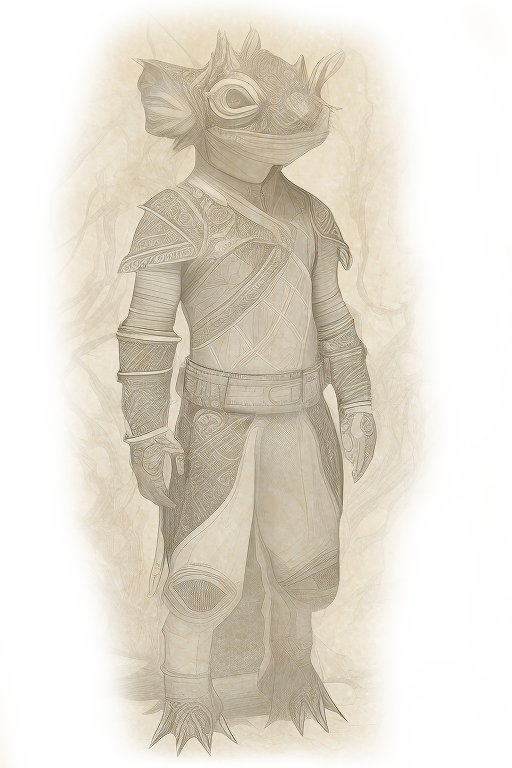
\includegraphics[height=\textheight/4,keepaspectratio]{images/kreek_sketch.png}
    \begin{DndReadAloud}
        Kreek in his leather armour created by Leon.
    \end{DndReadAloud}
\end{center}


\newpage

\subsection*{Leaving Tarreton}
When Leon came back and showed us the armour he created for Kreek! He looked like a cute new kobold. We wanted to rent a horse from HTS Pony but Nevrest was acting up.

Deciding not to tempt him, we left on foot.

When we walked past the ruins of the arena, Leon and Meirah overheard two peasants talking about the arena. "What a shame it was destroyed", enraged they threatened them and told them we were kept against our will. What an emotional outburst of them.

Nevrest took it to a whole level and I felt the weave being disturbed while he \textit{suggested} the one guy keeps on drinking and drinking. While running off we saw him drink from every container, even the vase.

\subsection*{HTS Pony}
After making camp, Nevrest felt compelled to tell the whole story about HTS pony. HTS stands for "Henry Morren, Tha'dad Earthfinger, Stod Pairhoof".

Henry, Nevrest said, is a \textbf{thief} and a \textbf{thug}. Nevrest first name is Thomas, and his family used to be a wealthy, owning a successful fishing company.

Nevrest sister husband, Anton, was desperate to make something out of himself and made a deal with Henry detailing that when something would happen to Anton, or his successors/family Henry would inherited the whole Nevrest company.

Not long after a fire killed almost the whole family, besides Clara. Clara was the daughter of Nevrest sister. After Thomas was able to protect and secure his cousin, he went to confront Henry in one of his illegal fishing companies. Nevrest was manhandled and thrown with the sharks. That's why he has those scars.

This all happened some years ago, but he doesn't talk much about it.

\subsection*{Big bad wolf}
While I was in my trance, a big dire wolf and 4 smaller ones attacked our camp. We were able to slay the beasts and even skin some. Leon now has some hides and we have meat to cook.
